\chapter{性能测试}
\begin{figure}[htbp]
\centering
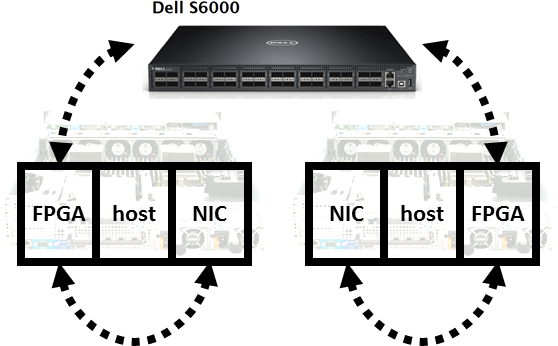
\includegraphics[width=4in]{connect}
\caption{实验环境示意} \label{fig:connect}
\end{figure}
我们在运行Windows Server 2012 R2的戴尔R720服务器上评估ClickNP的性能。
FPGA通过以太网端口与机架顶(top-of-rack, ToR)的戴尔S6000交换机\cite{s6000}相连。
如图~\ref{fig:connect} 所示,主机通过网卡发出的RDMA包,经FPGA丢包及记录,由交换机到达接收端。

我们在主机上运行ndping、ndrping等程序,进行RDMA读、写、发送等数据操作,
测量其通信带宽及延迟,并与PCIe接口通信进行对比。

\begin{figure}[htbp]
\centering
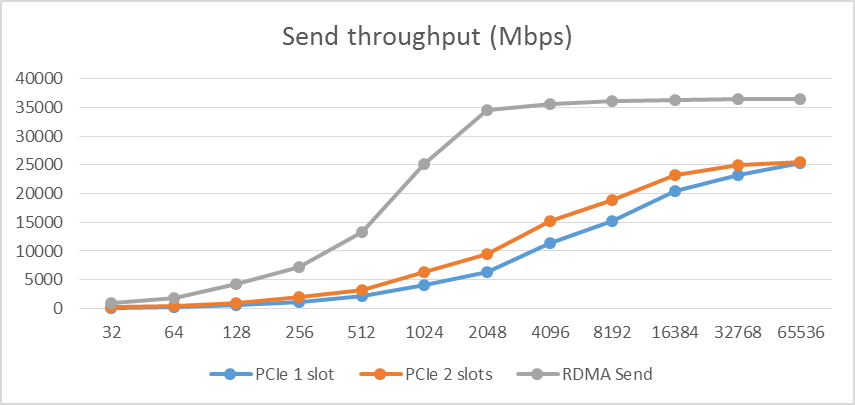
\includegraphics[width=4in]{rocerate}
\caption{RDMA Send与PCIe接口通信带宽对比} \label{fig:rocerate}
\note{实验中Send、Read、Write的性能没有明显差异,故只列出Send的数据}
\end{figure}

据图~\ref{fig:rocerate} 可见,随着包的增大,单位时间内需要处理的包数目减少,
系统从计算密集向数据密集转变,PCIe与RDMA均达到其带宽上限。
RDMA的通信带宽为40Gbps(实际中为36Gbps),高于PCIe接口的32Gbps(实际中25.6Gbps)。

\begin{figure}[htbp]
\centering
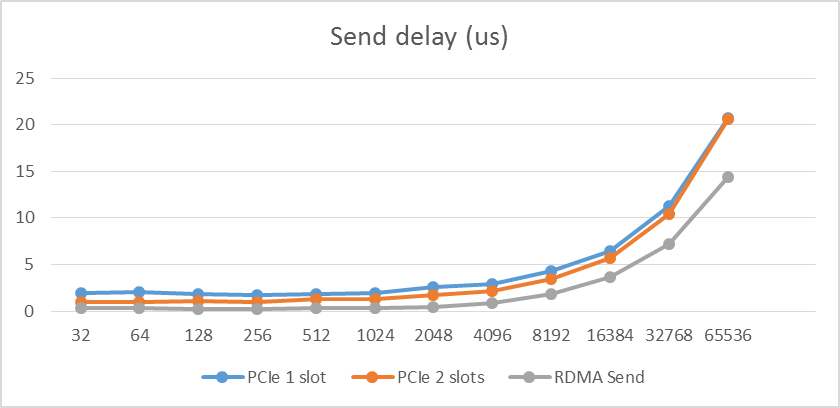
\includegraphics[width=4in]{rocelat}
\caption{RDMA Send与PCIe接口通信延迟对比} \label{fig:rocelat}
\end{figure}

\begin{figure}[htbp]
\centering
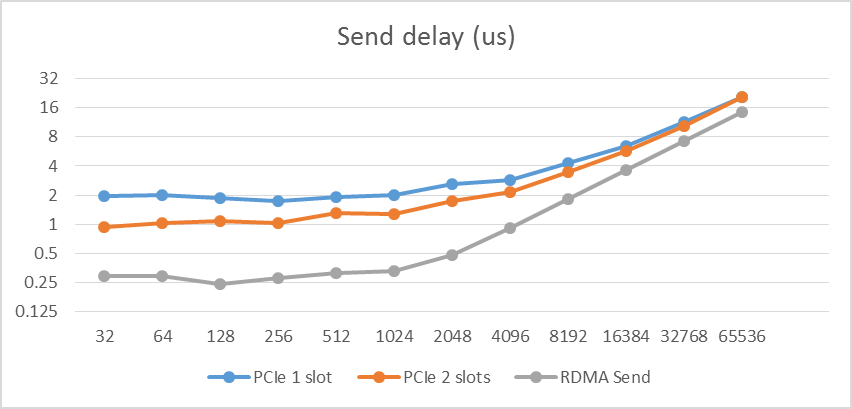
\includegraphics[width=4in]{rocelatlog}
\caption{RDMA Send与PCIe接口通信延迟对比(对数纵坐标)} \label{fig:rocelatlog}
\end{figure}

据图~\ref{fig:rocelat}、图~\ref{fig:rocelatlog}可见,随着包的增大,帧数增多,
处理所需的周期数线性增加,在通信延迟上也得到了体现。

实验结果表明,RoCE能够有效利用网卡的通信带宽,实现比PCIe接口更高的传输速率以及更低的延迟。
使用RoCE替代PCIe通信能够提升FPGA的存储性能。
